Ne interesează să găsim \textit{cea mai bună strategie}. Pentru a compara între ele mai multe strategii, trebuie să gândim \textit{un mediu în care acestea să concureze}. 
 
Până la a găsi cea mai bună strategie, trebuie, mai întâi, să vedem cum anume poate configurația unui algoritm genetic să influențeze calitatea soluției. De asemenea, vrem să vedem cum anume se comportă într-un mediu de test strategia propusă de algoritm. 
 
Pentru a îndeplini aceste cerințe, am ales să supun cromozomii la un anumit tip de turneu, ce poartă denumirea de \textbf{turneu cu eliminare}.  

\section {Termeni întâlniţi}
O \textbf{rundă} este dată de alegerea, în mod secret, a mișcării următoare și actualizarea scorului în funcție de ce a pus și oponentul. 

Un \textbf{meci} este jucat de către doi jucători. Este alcătuit dintr-un număr de runde. În fiecare rundă, fiecare jucător alege, în mod secret, ce mișcare va face. La final de rundă, scorul jucătorilor este actualizat cu o valoare dată de mișcarea făcută de fiecare, în funcție de ce a ales și oponentul să facă. 

\section {Cum este modelat un turneu cu eliminare}
 
Un turneu cu eliminare pornește de la o populație de strategii în care, la fiecare iterație, fiecare individ joacă câte un meci cu ceilalți indivizi. Pe parcursul meciurilor, câștigurile individuale se însumează într-un scor total. După ce se joacă toate combinările de doi jucători (se ajunge la finalul iterației), se elimină un procent din cei mai slabi jucători.  Pentru a mai reduce din numărul parametrilor ale căror valori pot varia, am stabilit că procentul să fie de 25\%. În caz de egalitate a scorurilor între doi jucători, se elimină la întâmplare unul din cei doi. Se completează locurile eliberate cu stategii care au obținut printre cele mai bune scoruri. Se resetează scorul total al indivizilor și se repetă acești pași până când în turneu a rămas un singur tip de strategie, ori până când am atins un număr maxim de iterații.  
\\\\
\textit{Observație}: Când într-un turneu cu eliminare concurează doi indivizi ce au aceeași strategie deterministă, la finalul unei iterații, cei doi indivizi vor avea exact același scor. Nu putem spune același lucru despre doi indivizi care folosesc strategia \textbf{Random}.
\\\\
Pentru a vedea clar modul în care evoluează strategiile în contextul acestui tip de turneu, am implementat o metodă grafică de vizualizare a datelor. Am ales să folosesc \textbf{line chart}-uri. Axa absciselor are drept legendă numărul de indivizi din fiecare strategie. Axa ordonatelor reprezintă indexul rundei turneului.

\section {Concluzii trase în urma finalizării turneelor}

Fiecare experiment este dat de stabilirea parametrilor configurației algoritmului genetic, urmată de rularea algoritmului genetic și trecerea soluției prin mai multe medii de testare, prin varierea configurației turneului cu eliminare.

În contextul acestei probleme, nu putem vorbi despre optim local sau global, întrucât un fitness cu o valoare bună obținut pentru un cromozom în faza de antrenare poate să își piardă relevanța în faza de testare datorită faptului că mediul de testare poate varia. 

În rândurile următoare prezint o serie de experimente.  

\subsection {Explorarea redusă a spațiului de căutare} 

\begin{center}
	\underline{\textit{Experimentul 1}}
\end{center}

\textit{Configurația algoritmului genetic și cea a turneului cu eliminare este trecută în \textbf{Anexa numărul 1}}.\\

Am făcut un prim experiment în care configurația algoritmului genetic a dus la o explorare redusă a spațiului de căutare. Pentru aceasta, am ales valori mici pentru numărul de generații, pentru numărul de runde din turneul clasic și pentru probabilitățile operatorilor genetici.
 
Diagramele de mai jos atestă calitatea redusă a soluției obținute în urma experimentului. 

\begin{figure}[H]
	\centering
	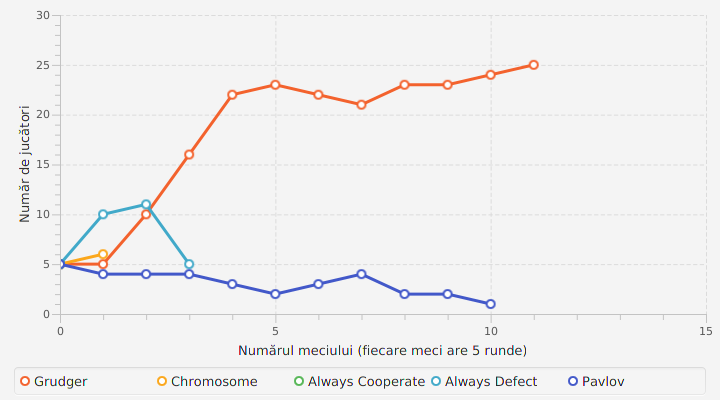
\includegraphics[	
	width=16cm,
	height=7.5cm,
	keepaspectratio
	]{imagini/experiment_1_epoch_1529303072346/chart_from_epoch_1529303304972.png}
	\caption{}
\end{figure}

\begin{figure}[H]
	\centering
	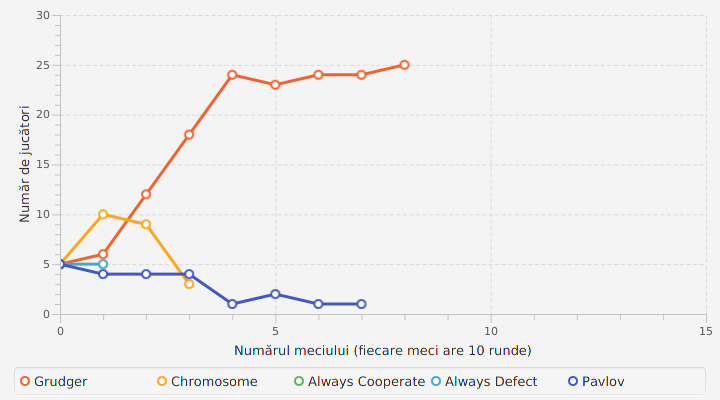
\includegraphics[	
	width=16cm,
	height=7.5cm,
	keepaspectratio
	]{imagini/experiment_1_epoch_1529303072346/chart_from_epoch_1529303340019.png}
	\caption{}
\end{figure}

\begin{figure}[H]
	\centering
	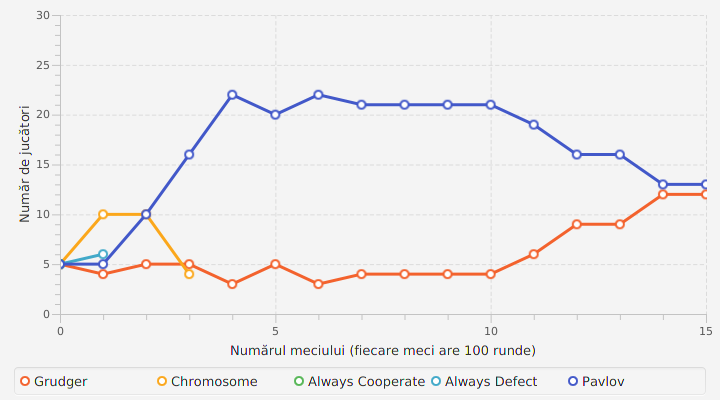
\includegraphics[	
	width=16cm,
	height=7.5cm,
	keepaspectratio
	]{imagini/experiment_1_epoch_1529303072346/chart_from_epoch_1529303352244.png}
	\caption{}
\end{figure}

\begin{figure}[H]
	\centering
	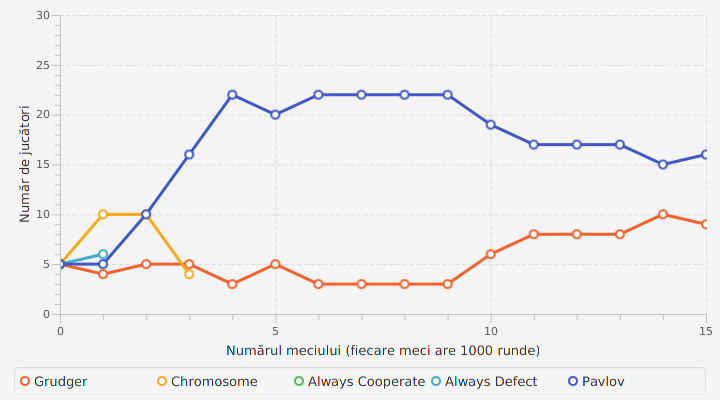
\includegraphics[	
	width=16cm,
	height=7.5cm,
	keepaspectratio
	]{imagini/experiment_1_epoch_1529303072346/chart_from_epoch_1529303371162.png}
	\caption{}
\end{figure}

\subsection {Numărul de runde al meciurilor din turneul cu eliminare}

\begin{center}
	\underline{\textit{Experimentul 2}}
\end{center}

\textit{Configurația algoritmului genetic și cea a turneului cu eliminare este trecută în \textbf{Anexa numărul 2}}.\\

Într-un alt experiment, am surpins cum numărul de runde, odată modificat cu o valoare foarte mică, a avantajat una din strategiile algoritmului genetic. 

\begin{figure}[H]
	\centering
	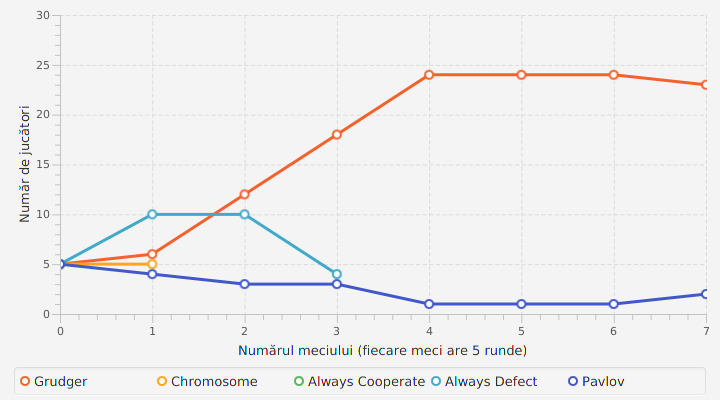
\includegraphics[	
	width=16cm,
	height=7.5cm,
	keepaspectratio
	]{imagini/experiment_2_epoch_1529309949939/chart_from_epoch_1529310422567.png}
	\caption{}
\end{figure}

\begin{figure}[H]
	\centering
	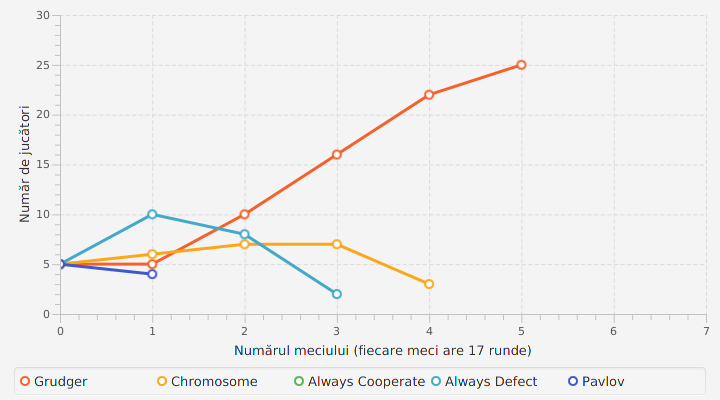
\includegraphics[	
		width=16cm,
		height=7.5cm,
		keepaspectratio
	]{imagini/experiment_2_epoch_1529309949939/chart_from_epoch_1529310399495.png}
	\caption{}
\end{figure}

Mărind cu 1 numărul de runde din fiecare meci, observăm că strategia propusă de algoritmul genetic câștigă. 

\begin{figure}[H]
	\centering
	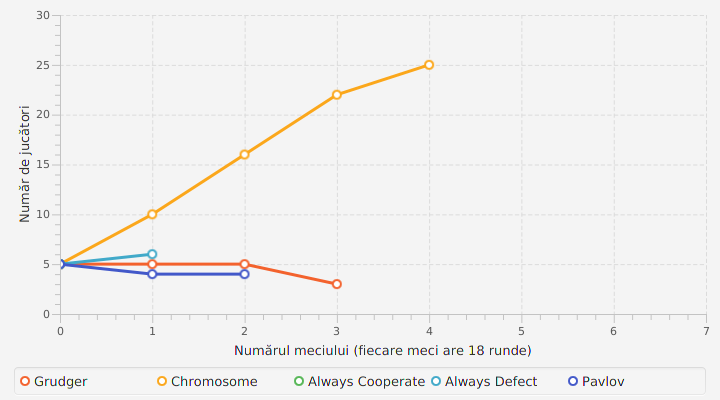
\includegraphics[	
	width=16cm,
	height=7.5cm,
	keepaspectratio
	]{imagini/experiment_2_epoch_1529309949939/chart_from_epoch_1529310386663.png}
	\caption{}
\end{figure}

\subsection{Strategia \textbf{Random}}

\begin{center}
	\underline{\textit{Experimentele 3 și 4}}
\end{center}

\textit{Configurația algoritmului genetic și cea a turneului cu eliminare este trecută în \textbf{Anexa numărul 3}}.\\
 
Strategia \textbf{Random} nu reprezintă o problemă pentru strategiile oferite de algoritmul genetic.

Am antrenat o populație de dimensiune mică (15 indivizi) într-un număr de 1000 de generații, lansând valori mari ale mutației și încrucișării (50\% pentru ambii operatori genetici). Populația de antrenament este dată de un singur individ de tip \textbf{Random}. Am rulat două experimente în urma cărora am obținut două strategii: într-un experiment numărul de runde ale turneului clasic a fost mic (5 runde) iar în celălalt a avut o valoare mai mare (100 de runde).

Pentru prima strategie obtinuta, numarul de runde al tuneului clasic este mai mic (5 runde). Pentru celalalt experiment, numarul de runde al tuneului clasic este 100.

În cele mai nefavorabile cazuri s-a ajuns la remiză.

\begin{figure}[H]
	\centering
	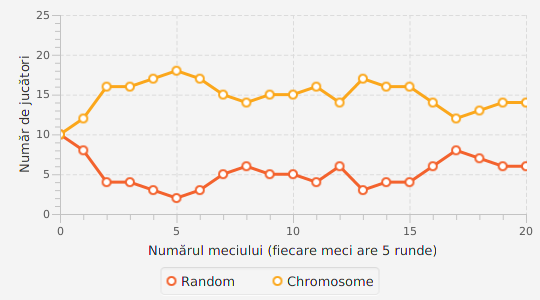
\includegraphics[	
	width=16cm,
	height=7.5cm,
	keepaspectratio
	]{imagini/chart_from_epoch_1529163979087.png}
	\caption{\textit{Exemplu de remiză.}}
\end{figure}

În rest se remarcă cum populația de cromozomi, în mare parte din evoluția sa, este în creștere și, la final, domină turneul cu eliminare.  

\begin{figure}[H]
	\centering
	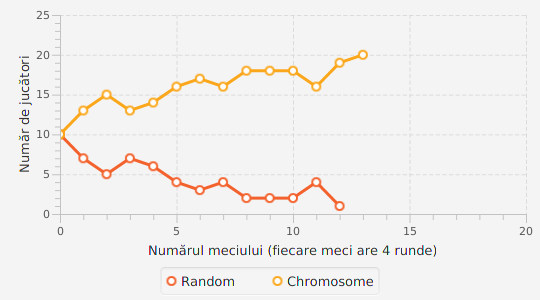
\includegraphics[	
	width=16cm,
	height=7.5cm,
	keepaspectratio
	]{imagini/chart_from_epoch_1529164104597.png}
	\caption{}
\end{figure}

\begin{figure}[H]
	\centering
	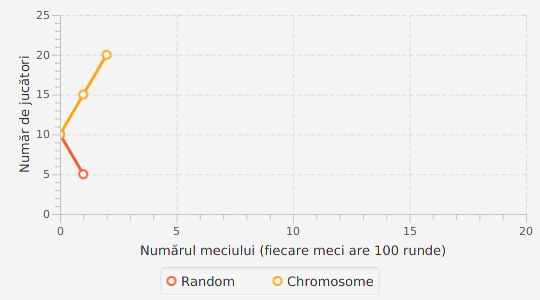
\includegraphics[	
	width=16cm,
	height=7.5cm,
	keepaspectratio
	]{imagini/chart_from_epoch_1529164689818.png}
	\caption{}
\end{figure}

\subsection{Relevanța populației de antrenament când populația de testare e diversificată}

Consider că \textbf{o populație diversificată de antrenament} poate simula condițiile din faza de testare. Din acest motiv am optat pentru ca aceasta să cuprindă fiecare strategie deterministă prezentată la secțiunea de strategii standard (am omis strategia \textbf{Random}). Prezența strategiei \textbf{Random} în faza de antrenament nu ajută la interpretarea calității soluției. Sunt șanse ca acestă strategie nedeterministă să obțină un scor bun în faza de antrenament, însă să nu facă față în faza de testare. 

Am pus câte un individ din fiecare strategie.

Am încercat să antrenez strategiile în contextul în care populația de antrenament era alcătuită doar din \textbf{Always Cooperate}, sau doar din \textbf{Always Defect}, sau doar din Tit-For-Tat, însă aceste strategii nu s-au comportat într-un mod notabil în faza de testare cand .

Un lucru ce se observă ușor este că strategia \textbf{Tit-For-Tat} reușește să câștige aproape de fiecare dată când la initiaizarea turneului cu eliminare toate strategiile au ponderi egale si numarul de runde este mare.

Strategia Tit-For-Tat poate totuși fi totuși bătută. Un astfel de context presupune ca strategiile cu care concurează să aleagă ca la fiecare pas să repete aceeași mișcare, asemeni strategiilor Always Defect și Always Cooperate. Motivul eliminării ar fi că la scoruri egale, când se dorește eliminarea unui singur jucător din 2 candidați, alegerea se face la întâmplare. Acest scenariu presupune schimbarea structurii populației de test. Observația este prezentată în exemplul de mai jos: 

\begin{figure}[H]
	\centering
	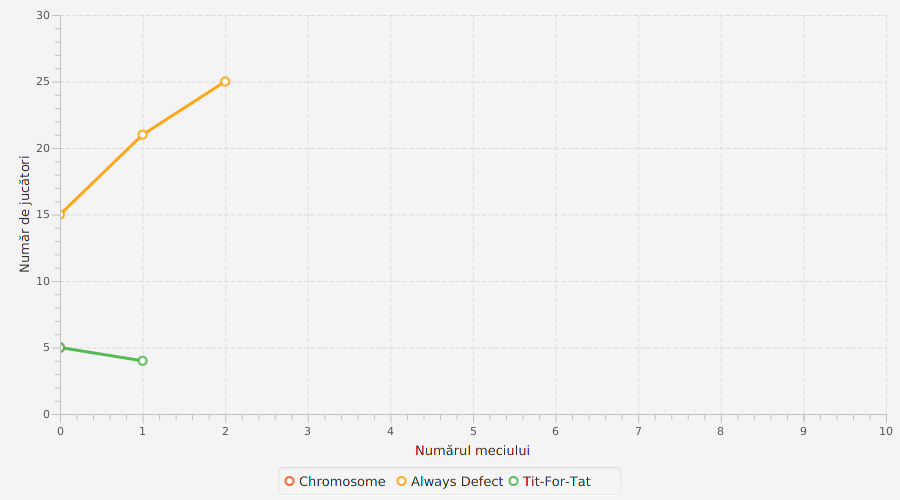
\includegraphics[	
	width=16cm,
	height=7.5cm,
	keepaspectratio
	]{imagini/chart_from_epoch_1528914497347.png}
	\caption{\textit{Strategia \textbf{Tit-For-Tat} pierde.}}
	\label{fig:tit_for_tat_pierde}
\end{figure}

Dacă vrem ca în exemplu să includem un cromozom și facem astfel încât strategia \textbf{Tit-For-Tat} să câștige, trebuie să defavorizam cromozomul lăsând numărul de runde la o valoare mică, cum ar fi 5. Dacă ar fi o valoare mai mare, în prima instanță s-ar elimina strategia care repetă aceeași mișcare, ca mai apoi să fie eliminate copiile cromozomilor. 























































































































































































































